% !TeX program = xelatex
% Code Agent + MiniOneRec variant. Original version: main.tex.
\documentclass[9pt,a4paper,fontset=fandol]{ctexart}
\usepackage[top=1.0cm,bottom=0.95cm,left=1.05cm,right=1.05cm]{geometry}
\usepackage{graphicx,xcolor,enumitem,titlesec,tabularx,hyperref}
\definecolor{resumeBlue}{HTML}{2457A6}
\pagestyle{empty}\setlength{\parindent}{0pt}\setlength{\parskip}{1pt}
\titleformat{\section}{\large\bfseries\color{resumeBlue}}{}{0pt}{}[\vspace{-5pt}\titlerule]
\titlespacing*{\section}{0pt}{6pt}{4pt}
\setlist[itemize]{leftmargin=1em,itemsep=1pt,topsep=1pt,parsep=0pt}
\hypersetup{hidelinks}
\begin{document}
\fontsize{8.8}{11.5}\selectfont
\begin{minipage}{0.82\textwidth}
{\LARGE\bfseries 李昕潼}\\[8pt]
18543740228\quad |\quad \href{mailto:xintong.li@u.nus.edu}{xintong.li@u.nus.edu}
\end{minipage}\hfill
\begin{minipage}{0.12\textwidth}\raggedleft
\IfFileExists{assets/resume_photo.png}{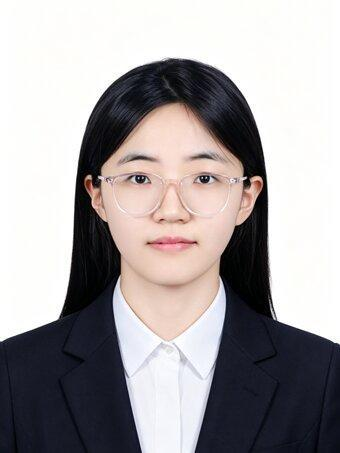
\includegraphics[width=1.65cm]{assets/resume_photo.png}}{}
\end{minipage}

\section{教育背景}
\begin{tabularx}{\textwidth}{@{}Xr@{}}\textbf{新加坡国立大学　计算机硕士（MComp）} & 2026/08--至今\end{tabularx}
\begin{tabularx}{\textwidth}{@{}Xr@{}}\textbf{北京邮电大学　通信工程本科} & 2022/09--2026/06\end{tabularx}
本科期间均分90.47，专业排名前5\%；获国家奖学金，获评北京市优秀毕业生。\par
\section{实习经历}
\begin{tabularx}{\textwidth}{@{}Xr@{}}\textbf{快手　AI Agent开发工程师（Code Agent方向）} & 2026/05--2026/07\end{tabularx}
{\small LangGraph / OpenCode / Context Engineering / Style Memory / Test-Time Scaling}\par
参与面向设计稿到可交互应用的Code Agent研发，围绕结构化上下文、分层任务规划、设计风格记忆与推理时迭代优化，改进多页面代码生成流程与效果。\par
\begin{itemize}
\item \textbf{上下文工程（Context Engineering）：}针对Figma节点逐层展开与多页面长上下文下生成效果不佳的问题，将布局、组件、样式及设计资源组织为页面级结构化表示，结合任务工作区按需加载，优化模型的设计理解与生成上下文。
\item \textbf{分层任务规划（Hierarchical Planning）：}基于LangGraph将复杂任务拆解为单页面实现、跨页面联动与交互动效补全等阶段，持久化页面上下文与生成产物，支持阶段间信息复用及多页面任务的连续推进。
\item \textbf{面向自进化的风格记忆（Style Memory）：}保存并复用设计师的设计风格信息，将历史偏好作为后续任务的生成条件，与当前设计上下文共同指导代码生成，支持跨任务偏好积累与个性化风格一致性。
\item \textbf{推理时优化（Test-Time Scaling）：}基于OpenCode串联代码生成、执行反馈与多轮修复，利用运行报错指导后续代码修正；分析尺寸异常、字体缺失和布局偏差等失败案例，迭代上下文组织与生成策略。
\end{itemize}
\section{项目经历}
\begin{tabularx}{\textwidth}{@{}Xr@{}}\textbf{MiniOneRec：生成式推荐系统｜项目负责人} & 2026/08--2026/10\end{tabularx}
{\small Python / Sentence-BERT / RQ-VAE / Qwen2.5 / SFT / GRPO / DeepSpeed ZeRO-2}\par
面向传统推荐系统依赖ID嵌入、难以迁移语义知识的问题，构建端到端生成式推荐框架，将商品语义压缩为离散语义ID，通过大语言模型完成序列生成与偏好对齐。\par
\begin{itemize}
\item \textbf{语义ID构建与约束解码：}使用Sentence-BERT联合编码商品标题与描述，经三层RQ-VAE残差量化生成层次化语义ID（SID）；针对量化碰撞进行迭代去重，并结合约束解码限定合法商品空间，生成SID合法率达100\%。
\item \textbf{多任务监督微调（SFT）：}基于Qwen2.5将用户历史交互转为SID序列，联合语言建模与SID对齐目标开展next-token预测；使用DeepSpeed ZeRO-2在8×A100上完成分布式训练，降低显存占用并加速收敛。
\item \textbf{推荐导向的强化学习（GRPO）：}设计融合命中正确性与排序感知的复合奖励，对SFT模型进行GRPO策略优化；推理阶段结合约束束搜索（Constrained Beam Search），输出合法且去重的推荐候选。
\item \textbf{实验结果：}在Amazon Industrial \& Scientific数据集上，相较传统ID推荐模型，Recall@10提升15.2\%，NDCG@10提升12.8\%。
\end{itemize}
\begin{tabularx}{\textwidth}{@{}Xr@{}}\textbf{基于大模型智能体的网络故障根因定位系统} & 2025/12--2026/03\end{tabularx}
{\small Python / Qwen2.5-7B-Instruct / PEFT / LoRA / GRPO / LangChain / ReAct / RAG}\par
面向网络运维故障定位，结合结构化指标、知识检索与多步推理，实现从观测信息到候选根因的自动化诊断。\par
\begin{itemize}
\item \textbf{设计两阶段蒸馏式SFT数据流程：}基于TeleLogs，围绕工程参数、用户观测指标、症状描述与候选根因构建2,400条样本；先以排除、矛盾、规则、统计四类专家策略生成推理轨迹，再由教师模型整合、压缩与标准化正确轨迹，形成高质量RCA训练数据。
\item \textbf{开展参数高效训练与策略优化：}使用PEFT/LoRA对Qwen2.5-7B-Instruct进行监督微调，进一步结合GRPO优化最终根因判别，提升复杂故障场景下的输出稳定性与决策准确率。
\item \textbf{构建ReAct诊断智能体：}基于LangChain封装表格解析、故障区间识别、服务小区几何及邻区干扰分析工具，将原始数据转为结构化诊断证据；结合规则知识库与RAG开展多步推理，增强诊断的可解释性。
\item \textbf{实验结果：}Pass@1由基础模型的12.04\%提升至微调后的53.59\%，引入Agent后达到76.50\%；Pass@4对应由12.50\%提升至54.86\%和78.36\%。
\end{itemize}
\begin{tabularx}{\textwidth}{@{}Xr@{}}\textbf{CADDesigner：基于通用智能体的CAD模型设计系统} & 2025/06--2025/09\end{tabularx}
{\small Python / LangChain / Claude Sonnet / CadQuery / PythonOCC / ReAct / Function Calling}\par
面向非专业用户，实现文本或参考图片到CAD代码生成、模型构建、三视图渲染与迭代修复的完整闭环。\par
\begin{itemize}
\item \textbf{设计智能建模工作流：}基于LangChain组织需求解析、代码生成、模型构建、渲染、视觉评估与迭代修复，通过多步推理与工具调用持续优化生成结果。
\item \textbf{实现多模态理解与代码生成：}使用Claude Sonnet联合理解文本描述和参考图像，提取几何特征、结构关系及建模约束，生成CadQuery/PythonOCC参数化建模代码。
\item \textbf{构建视觉反馈迭代修复机制：}在sandbox中执行代码、构建3D模型并渲染标准三视图，将结果反馈给Agent评估视觉一致性；若与需求存在偏差，则修正或重新生成代码并进入下一轮闭环。
\item \textbf{实验结果：}在CAD-VGDrawing上取得IoU 0.2769、CD 0.1097、HD 0.4347，有效模型生成成功率（SUC）100.0\%。
\end{itemize}
\section{技能特长}
开发环境：Linux、Shell、Git、Conda、远程GPU服务器。\par
模型训练：LoRA/QLoRA、PEFT、GRPO；数据构建、领域微调与效果评测。\par
智能体开发：LangGraph、LangChain、ReAct、Tool Calling、Multi-Agent。\par
\end{document}